\documentclass[pdftex, 12pt, a4paper]{article}

\usepackage[pdftex]{graphicx}
\usepackage[utf8x]{inputenc}
\usepackage{appendix}
\usepackage{cite}
%\usepackage{pgfgantt}
%\usepackage{pst-gantt}
\usepackage{rotating}
\usepackage{pdflscape}
\usepackage{hyperref}
%\usepackage{breakurl}
\usepackage{listings}
\usepackage{nomencl}
\usepackage[a4paper]{geometry}
\usepackage{tabularx}
\usepackage{longtable}

\nomitemsep 1pt

\makenomenclature

\begin{document}

\begin{titlepage}

\begin{center}

{\large Electronics and Computer Science\\
Faculty of Physical and Applied Sciences\\
University of Southampton}\\[5em]

{\LARGE On the Implementation of Authentication Mechanisms for Mobile Devices over Wireless Networks}\\[5em]

{\large Thomas Grainger}\\[5em]

{\large \today}\\[5em]


\end{center}

\end{titlepage}


\tableofcontents

\begin{abstract}
The IEEE 802.1X authentication standard has become one of the most well used architectures for wireless authentication where it is required to support a number of distinct users who can authenticate independently of each other (in contrast to pre-shared key based methods of authentication).  The primary objective of this project is to ``design and demonstrate a simulation of the implementation of an efficient authentication protocol for mobile networks'' specifically an example of 802.1X using the RADIUS protocol for Authenticator-to-Authentication Server communications in a simulated environment, then further demonstrate the system in reality on multiple wireless Access Points (APs). A further goal of the project is to investigate the use of 802.11r as a method to allow fast roaming between those APs.
\end{abstract}
\nomenclature{AP}{Access Point}

\section*{Acknowlegements}
\addcontentsline{toc}{section}{Acknowledgments}
\begin{itemize}
  \item Southampton University Wireless Society (SUWS).
  \item PaulFertser and the other members of \verb`#linux-wireless` on \verb`irc.freenode.net`.
  \item Tom Blount, José Cubero and Chris Orchard the other members of ELEC6076 Wireless Networks group B.
\end{itemize}
\nomenclature{SUWS}{Southampton University Wireless Society}

\section{Introduction}
As networks have begun to allow multiple people to connect, secure systems have been developed to allow this.  While authorization is useful on any network it is particularly important in wireless networks where there is no physical protection of the network. The simplest method is to configure a single PSK\nomenclature{PSK}{pre-shared key} and issue it to every user to authorize them to use the network. The obvious issue with a single PSK is that users cannot easily have their network authorization revoked without re-issuing a new key to every other user.

The IEEE 802.1X standard was created to address the constraints of PSK. It controls access to the network in a way that supports a number of distinct users who authenticate independently of one another. As the users are authenticated individually, a network administrator has a greater degree of control on who can access the network. In addition to the ease of granting and revoking network access, this system allows administrators to track an individual's resource usage.  This project aims to investigate an implementation of this standard both in practice and in simulation.

\section{Background}
\subsection{IEEE 802.1X}
IEEE 802.1X the IEEE Standard for controlling access to wireless and wired LANs\nomenclature{LAN}{Local Area Network} operates by encapsulating EAP over LAN (EAPOL).  The 802.1X authentication process requires three components: the authentication server, the authenticator and the supplicant.  The diagram below shows the structural elements of 802.1X and how EAP is tunneled via EPOL to the authenticator, and then via the Remote Authentication Dial In User Service, RADIUS or Diameter protocols to the authentication server. Although in this project 802.11 wireless Ethernet is used in place of the wired Ethernet shown in Figure \ref{fig:img-1}.

\begin{figure}[htb]
\centering
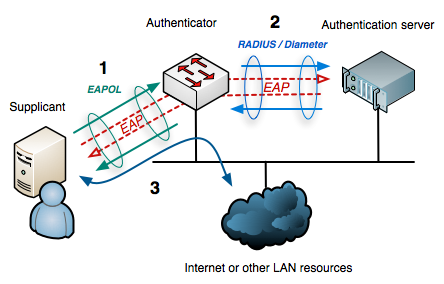
\includegraphics[width=0.8\textwidth]{img/8021X.png}
\caption{802.1X wired protocols \protect\cite{8021X-diag}}
\label{fig:img-1}
\end{figure}

\nomenclature{EAPOL}{EAP over LAN}
\nomenclature{EAP}{Extensible Authentication Protocol}

\subsubsection{Authentication Server}
The authentication server is used to store credentials, authenticate users given those credentials and track usage of resources; this is known as ``authentication, authorization and accounting'' or AAA\cite{RFC2865,RFC2866}.  The authentication server can either proxy the request to a different server based on a user's realm, query an LDAP database, or as is the case in this project be hard configured in the authentication server's configuration file.

In this project the only features used are authentication and authorization, resource usage is outside of the scope of this project.

\subsubsection{Authenticator}
The authenticator is installed on a switch or wireless AP and `guards' a protected network.

Unless 802.1X authentication has been completed, the authenticator will not route any non-EAP packets to the protected areas of the network\cite{8021X-book}. This is in contrast to the captive portal authentication system, also known as web redirection, where clients must be provided with access to the network and allocated an IP address as part of the authentication process\cite{wifi-dog}.

When operating over a wireless network instead of authorizing a particular port as in wired Ethernet a WPA\nomenclature{WPA}{Wi-Fi Protected Access} PMK\nomenclature{PMK}{Pairwise Master Key} is allocated and authorized.  This is known as WPA-802.1X or WPA-Enterprise\cite{IEEE8021X-2004}.
\subsubsection{Supplicant}
The term ``supplicant'' is sometimes used to refer to a client device or station, or some software package on a client device used to communicate with and transmit authentication credentials to the authenticator.  Throughout this project, the term supplicant will be used to refer to the software package.
802.11r

When roaming between access points using WPA-PSK client stations are only required to re-generate a PTK\nomenclature{PTK}{Pairwise Transient Key} and GTK\nomenclature{GTK}{Group Temporal Key} from the PMK, generated from the PSK or pass-phrase, using a `four-way handshake'\cite{IEEE80211i-2004}.  In comparison when using WPA-802.1X the client station must obtain a PMK via a complete 802.1X authentication process every time time it roams to a new access point, this process can be fairly time consuming and can cause noticeable degradation to network applications that require high availability and low latency, such as streaming media or VOIP \nomenclature{VOIP}{Voice Over  IP}\cite{voip-time}.  To solve this issue IEEE 802.11r-2008 or fast BSS transition (FT) allows a client station to roam between access points without needing to renegotiate a key with the 802.1X authentication server.

\nomenclature{FT}{fast BSS transition}
\nomenclature{BSS}{Basic Service Set}
\nomenclature{IP}{Internet Protocol}

\subsection{Software Tools}
As with all standards and protocols, multiple different implementations are available.  This section describes which packages were chosen and the justifications for these choices.

FreeRadius was chosen to implement the authentication server over other RADIUS and Diameter servers as it is the most popular and widely deployed authentication server available for Linux hosts.

The 802.1X authenticator chosen was `\verb`hostapd` running on Meraki Mini hardware donated for use in the project by SUWS as part of the Southampton Open Wireless Network (SOWN) project.  The firmware chosen to run on these Meraki nodes is OpenWrt, an open source Linux distribution specifically designed for embedded network devices. As the Meraki units were pre-2008 models, the installation of open source firmware was permitted and were not subject to the EULA change preventing installation of non-Meraki software on new Meraki hardware. While there are alternative open source firmware options available for installation on the Meraki Mini, they are either no longer being developed or are derivatives of OpenWrt\cite{meraki-eula}.

\nomenclature{EULA}{End User License Agreement}

All experiments simulating a system over a wired or local Unix socket connection the test program \verb`eapol_test` was used. All experiments using a real wireless network were conducted with Linux machines running `\verb`wpa_supplicant`'. These were selected as opposed to any of the closed source implementations as these did not provide the control over configuration and debug information required for the project; specifically the ability to force a client access point to roam between nodes.  The supplicant, \verb`wpa_supplicant`, it's controlling interfaces \verb`wpa_cli` and \verb`wpa_gui`, the authenticator \verb`hostapd` and the test program \verb`eapol_test` are all provided by a single project: `\verb`hostapd` and \verb`wpa_supplicant`' by Jouni Malinen et al\cite{wpa-hostapd}.

\section{Specification}
To aid in the task of designing a solution, a set of  requirements were drawn up with MOSCOW priority attached to each. These requirements were derived from the technical background research of the project.  Each of these tasks were then subdivided into further subtasks required to achieve that task.

\begin{itemize}
    \item Must: Demonstrate a simulation of 802.1X
    \begin{itemize}
        \item Configure a RADIUS authentication server on a virtual machine
        \item Simulate 802.1X using another process on that virtual machine using \verb`eapol_test`
    \end{itemize}
    \item Must: Demonstrate 802.1X working in reality with a wireless AP
    \begin{itemize}
        \item Flash an AP with OpenWrt
        \item Configure \verb`hostapd` in the AP
        \item Simulate 802.1X on the AP using \verb`eapol_test`
        \item Connect to the AP with a laptop using \verb`wpa_supplicant`
    \end{itemize}
    \item Should: Demonstrate 802.1X working with multiple APs
    \begin{itemize}
        \item Flash extra APs with OpenWrt
        \item Duplicate configuration
        \item Demonstrate a forced roam with \verb`wpa_cli` using a wireless enabled laptop
    \end{itemize}
    \item Could: Demonstrate 802.11r FT between those APs
    \begin{itemize}
        \item Recompile \verb`hostapd` to support 802.11r on the APs
        \item Configure an 802.11r wireless controller on one of the APs
        \item Recompile \verb`wpa_supplicant` to support 802.11r on a laptop
        \item Demonstrate a forced roam with \verb`wpa_cli` using a wireless enabled laptop
    \end{itemize}
\end{itemize}

\section{Implementation}
\subsection{RADIUS}
FreeRADIUS was deployed on a RHEL VMWare virtual machine, \verb`kanga-cso1g09e`, by installing the package \verb`freeradius` from the official RHEL package repositories.  A self-signed X.509 certificate key pair was generated, so as to be able to authenticate the RADIUS server to the client supplicant when using EAP-TTLS, although in this project the certificate was ignored because it was assumed that an MITM attack was too unlikely to occur in the short space of time while testing the system.

\nomenclature{RHEL}{Red Hat Enterprise Linux}
\nomenclature{EAP-TTLS}{EAP Tunneled Transport Layer Security}
\nomenclature{MITM}{Man In The Middle}

The specific configuration files that must be edited are: \verb`/etc/raddb/users`, to configure authorised users e.g. username ``TomB'' and password ``TomBsPassword''; \verb`/etc/raddb/clients.conf` to describe which authenticators are able to connect to what e.g. \verb`kanga-cso1g09e` and \verb`linuxproj` and finally \verb`/etc/raddb/eap.conf`, to configure the EAP-TTLS authentication protocol.  The listings of these files are available in the appendix.

To demonstrate that the radius server was working \verb`eapol_test` was compiled from source and executed on both \verb`kanga-cso1g09e` and \verb`linuxproj`.  \verb`eapol_test` requires a config file to define the credentials and authentication protocol type and configuration for testing. This file is listed in full in the appendix.

\subsection{hostapd and OpenWrt}
The OpenWrt operating system was cross compiled to Atheros AR231x/AR5312, the CPU architecture of the Merai Mini APs using the build instructions available on the OpenWrt website\cite{openwrt-build}. As well as the operating system, the OpenWrt build tools provide the ability to add packages and build a complete compilation toolchain for the ARM architecture.  The only packages added were the `\verb`hostapd` and \verb`hostapd-utils` packages.  The firmware image produced was then flashed onto both of the APs.

\nomenclature{CPU}{Central Processing Unit}

To allow the APs to access the authentication server they must be given access to the internal ECS network.  This was achieved by having a laptop connected to the internal ECS network via the undergraduate VPN server \verb`ugvpn`, this laptop shared its single globally routable IP address in the 152.78.236.0/24 subnet via NAT to IP addresses allocated in the 10.42.0.0/16 subnet.  The APs are then allocated IPs in the 10.42.0.0/16 subnet via a DHCP server running on the laptop.

\nomenclature{VPN}{Virtual Private Network}
\nomenclature{NAT}{Network Address Translation}

    % TODO: see config files
    % TODO: \verb`eapol_test` cross compile

\subsection{supplicant and 8021.X experiment}
While it was possible to demonstrate 802.1X working using a single AP at this stage simply by connecting to the ``notthebees'' wireless network from the built in network management tools of various wireless client devices: an Android device, a Fedora Linux laptop and a Ubuntu laptop; it is very difficult to demonstrate that the supplicant can connect to both APs and roam between them from these GUI interfaces.

Both Ubuntu and Fedora provide \verb`wpa_supplicant` by default and configure it automatically using network-manager: a more user friendly interface to wireless configuration.  Rather than allowing network-manager to control \verb`wpa_supplicant` a configuration file, \verb`wpa_supplciant.conf`, was created. This configuration file, while very similar to the \verb`hostapd` configuration with the authentication details required by the protocol, also includes the configuration required by the wireless network - specifically the encryption types for the GTK and PTK and the SSID.  To force the client machine to roam between the different APs the \verb`wpa_cli` command ``roam <BSSID>'' was issued.  The full output of a successful roam is available in the appendix.
802.11r

\nomenclature{BSSID}{BSS Identifier}
\nomenclature{SSID}{Service Set Identifier}

    % TODO: How to configure on different sections
    % TODO:    On controller
    % TODO:    On access points
    % TODO:    On client supplicant, FT-EAP
    % TODO: \verb`wpa_cli` roam

When \verb`wpa_supplicant` was configured with FT-EAP the debug information from \verb`wpa_cli` showed that the connection was unsuccessful.

At \verb`rsn_supp/wpa_ft.c` line \verb`00152`, the ``Group Suite Selector'', the group cipher type should be one of \verb`WPA_CIPHER_CCMP` or \verb`WPA_CIPHER_TKIP`.  In the \verb`wpa_cli` debug information, however, we see ``FT: Invalid group cipher (0)'' which shows that the code is receiving an unexpected value of 0 or \verb`WPA_CIPHER_NONE` as defined in \verb`common/defs.h`.  Clearly this is not correct, both the \verb`hostapd` and \verb`wpa_supplicant` configuration requires CCMP encryption for both the GTK and PTK. There was not sufficient time to determine if the root cause of this issue was due to a software error in \verb`wpa_supplicant` or if it was a configuration error and as such this section of the project was unsuccessful in demonstrating an FT roam.

\section{Evaluation}
The Table \ref{tab:evaluation} relates to the goals in the specification and their status, either completed or not completed.

\begin{table}[!hb]
    \label{tab:evaluation}
    \begin{tabular}{|l|l|l|}
        \hline
        Priority & Goal                                                     & Status        \\ \hline
        Must     & Demonstrate a simulation of 802.1X                       & Completed     \\ 
        Must     & Demonstrate 802.1X working in reality with a wireless AP & Completed     \\ 
        Should   & Demonstrate 802.1X working with multiple APs             & Completed     \\ 
        Could    & Demonstrate 802.11r FT between those APs                 & Not Completed \\
        \hline
    \end{tabular}
\end{table}

Although it was not possible to demonstrate 802.11r FT between APs, possibly due to bugs in the implementation of \verb`wpa_supplicant`, overall the project was extremely successful: all the high priority goals and most of the goals overall set-out at the beginning of the project were completed.

\section{Individual Contribution}
Although this report was a piece of work produced by an individual, the project it describes was implemented as a group involving three other members: specifically Tom Blount, José Cubero and Chris Orchard.

My contribution spanned multiple components of the project.  The building of the OpenWrt image and toolchain for the Meraki Mini wireless APs, so as to compile \verb`eapol_test` for that platform.

Configuring \verb`wpa_supplicant` for 802.1X and 802.11r, performing the client part of the experiments for both regular 802.1X and 802.11r.  As part of these experiments performed I captured debug information that made it possible for me track down possible reasons for the failure of 802.11r.

%references
\addcontentsline{toc}{section}{References}
\bibliographystyle{IEEEtran}
\bibliography{final-report,rfc,i-d,tag1g09,cso1g09,nv2g09,wl15g09}{}

%Appendices
\appendix
\verbatiminput{appendix/foo.txt}
\section{List of Abbreviations}
\renewcommand{\nomname}{}
\printnomenclature

\clearpage

\section{RADIUS configuration}
\label{sec:Code;sub:radius}

\subsection{/etc/raddb/users}
\begin{verbatim}[frame=single]
#Give access to this user
TomB    Cleartext-Password := "TomBsPassword"
        Reply-Message = "Hello there %{User-Name}! How's it going?"

#Don't give access to this user
TomG    Auth-Type := Reject
        Reply-Message = "Oh no you don't Grainger. Not again."
\end{verbatim}

\subsection{/etc/raddb/clients.conf}
\begin{verbatim}[frame=single]
client linuxproj {
    ipaddr = 152.78.71.57
    secret = testing123
    require_message_authenticator = no
    
    #Used to specify a specific Network Access Server type
    #(e.g. cisco, multitech, etc.)
    nastype = other
}
\end{verbatim}

\subsection{/etc/raddb/eap.conf}
\begin{verbatim}[frame=single]
tls {
    certdir = ${confdir}/certs
    cadir = ${confdir}/certs
    private_key_password = whatever
    private_key_file = ${certdir}/server.pem
    certificate_file = ${certdir}/server.pem
    CA_file = ${cadir}/ca.pem
    dh_file = ${certdir}/dh
    random_file = ${certdir}/random
    CA_path = ${cadir}
    cipher_list = "DEFAULT"
}

ttls {
    default_eap_type = md5
    copy_request_to_tunnel = no
    use_tunneled_reply = no
    virtual_server = "inner-tunnel"
}
\end{verbatim}

\section{Authenticator}
\label{sec:Code;sub:authenticator}

\subsection{/etc/hostapd/hostapd.conf}
\subsubsection{802.1X}
%TODO: add stuff

\subsubsection{802.11r}
\begin{figure}[h!]
\begin{verbatim}[frame=single]
auth_server_addr=152.78.61.5
auth_server_port=1812
auth_server_shared_secret=testing123
disable_pmksa_caching=1
okc=0
nas_identifier=kanga-cso1g09e
eapol_key_index_workaround=1
ieee8021x=1
wpa_key_mgmt=FT-EAP WPA-EAP
auth_algs=1
wpa=2
wpa_pairwise=CCMP
ssid=notthebees
bridge=br-lan
wmm_enabled=1
bssid=00:18:0a:01:3f:38
ignore_broadcast_ssid=0
mobility_domain=a1b2
r0_key_lifetime=100000
r1_key_holder=000102030406
reassociation_deadline=1000
r0kh=00:18:0a:01:3f:3f kanga-cso1g09e
    000102030405060708090a0b0c0d0e0f
r1kh=00:18:0a:01:3f:3f 00:01:02:03:04:05
    000102030405060708090a0b0c0d0e0f
r1kh=00:18:0a:01:3f:38 00:01:02:03:04:06
    000102030405060708090a0b0c0d0e0e
\end{verbatim}
\caption{Configuration by Chris Orchard}
\end{figure}

\section{Supplicant}
\label{sec:Code;sub:supplicant}

\subsection{/etc/wpa\_supplicant/wpa\_supplicant.conf}
\subsubsection{802.1X}
\begin{figure}[h!]
\begin{verbatim}[frame=single]
ctrl_interface=/var/run/wpa_supplicant
eapol_version=1
ap_scan=1
fast_reauth=1

network={
        ssid="notthebees"
        scan_ssid=1
        key_mgmt=WPA-EAP
        pairwise=CCMP
        group=CCMP
        eap=TTLS
        identity="TomB"
        anonymous_identity="anon"
        password="TomBsPassword"
        phase2="auth=PAP"
}
\end{verbatim}
\end{figure}

\subsubsection{802.11r}
\begin{figure}[h!]
\begin{verbatim}[frame=single]
ctrl_interface=/var/run/wpa_supplicant
eapol_version=1
ap_scan=1
fast_reauth=1

network={
        ssid="notthebees"
        scan_ssid=1
        key_mgmt=FT-EAP WPA-EAP
        pairwise=CCMP
        group=CCMP
        eap=TTLS
        identity="TomB"
        anonymous_identity="anon"
        password="TomBsPassword"
        phase2="auth=PAP"
}
\end{verbatim}
\end{figure}

\newpage
\section{Testing Output}

\subsection{Simulation}
\label{sec:testing-output;sub:simulation}

\subsection{wpa\_supplicant output}
\subsubsection{802.1X}
\label{sec:testing-output;sub:supplicant}
\begin{figure}[h!]
\begin{verbatim}[frame=single]
<3>SME: Trying to authenticate with 00:18:0a:01:3f:38
    (SSID='notthebees' freq=2412 MHz)
<3>Trying to associate with 00:18:0a:01:3f:38
    (SSID='notthebees' freq=2412 MHz)
<3>SME: Trying to authenticate with 00:18:0a:01:3f:3f
    (SSID='notthebees' freq=2462 MHz)
<3>Trying to associate with 00:18:0a:01:3f:3f
    (SSID='notthebees' freq=2462 MHz)
<3>Associated with 00:18:0a:01:3f:3f
<3>CTRL-EVENT-EAP-STARTED EAP authentication started
...
<3>CTRL-EVENT-EAP-SUCCESS EAP authentication completed successfully
<3>WPA: Key negotiation completed with 00:18:0a:01:3f:3f
    [PTK=CCMP GTK=CCMP]
<3>CTRL-EVENT-CONNECTED - Connection to 00:18:0a:01:3f:3f
    completed (reauth) [id=0 id_str=]
> roam 00:18:0a:01:3f:38
OK
<3>SME: Trying to authenticate with 00:18:0a:01:3f:38
    (SSID='notthebees' freq=2412 MHz)
<3>Trying to associate with 00:18:0a:01:3f:38
    (SSID='notthebees' freq=2412 MHz)
<3>Associated with 00:18:0a:01:3f:38
<3>CTRL-EVENT-EAP-STARTED EAP authentication started
...
<3>CTRL-EVENT-EAP-SUCCESS EAP authentication
    completed successfully
<3>WPA: Key negotiation completed with 00:18:0a:01:3f:38
    [PTK=CCMP GTK=CCMP]
<3>CTRL-EVENT-CONNECTED - Connection to 00:18:0a:01:3f:38
    completed (reauth) [id=0 id_str=]
\end{verbatim}
\end{figure}

\subsubsection{802.11r}
\label{sec:testing-output;sub:80211r}
\begin{figure}[h!]
\begin{verbatim}[frame=single]
wlan0: Trying to associate with 00:18:0a:01:3f:38
    (SSID='notthebees' freq=2412 MHz)
FT: Invalid group cipher (0)
wlan0: Authentication with 00:18:0a:01:3f:38 timed out.
wlan0: Trying to associate with 00:18:0a:01:3f:3f
    (SSID='notthebees' freq=2462 MHz)
wlan0: Authentication with 00:18:0a:01:3f:3f timed out.
wlan0: Trying to associate with 00:18:0a:01:3f:3f
    (SSID='notthebees' freq=2462 MHz)
wlan0: Authentication with 00:18:0a:01:3f:3f timed out.
wlan0: Trying to associate with 00:18:0a:01:3f:38
    (SSID='notthebees' freq=2412 MHz)
^Cwlan0: CTRL-EVENT-TERMINATING - signal 2 received
\end{verbatim}
\end{figure}



\end{document}
